% Author: Izaak Neutelings (September 2020)
\documentclass[border=3pt,tikz]{standalone}
\usepackage{amsmath}
\usepackage{tikz}
\usepackage{physics}
\usepackage[outline]{contour} % glow around text
\usetikzlibrary{calc}
\usetikzlibrary{decorations.markings}
\usetikzlibrary{angles,quotes} % for pic
\usetikzlibrary{arrows.meta} % for arrow size
\usetikzlibrary{bending} % for arrow head angle
\usetikzlibrary{decorations.pathmorphing} % for decorate random steps
\tikzset{>=latex} % for LaTeX arrow head
\usepackage{xcolor}
\contourlength{1.3pt}

\colorlet{xcol}{blue!70!black!40}
\colorlet{xcol'}{xcol!50!red}
\colorlet{vcol}{green!45!black}
\colorlet{acol}{red!50!blue!80!black!80}
\tikzstyle{rvec}=[->,very thick,xcol,line cap=round]
\tikzstyle{vvec}=[->,very thick,vcol,line cap=round]
\tikzstyle{avec}=[->,very thick,acol,line cap=round]
\colorlet{myred}{red!65!black}
\tikzstyle{force}=[->,myred,very thick,line cap=round]
\tikzstyle{mass}=[line width=0.5,draw=red!50!black,fill=red!50!black!10,rounded corners=1,
                  top color=red!50!black!30,bottom color=red!50!black!10,shading angle=20]
\tikzstyle{disk}=[line width=0.5,orange!30!black,fill=orange!40!black!10,
                  top color=orange!40!black!20,bottom color=orange!40!black!10,shading angle=20]
\tikzstyle{pole}=[line width=0.5,blue!20!black,fill=orange!20!black!10,
                  top color=blue!20!black!20,bottom color=blue!20!black!10,shading angle=20]
\tikzstyle{rope}=[brown!70!black,line width=1,line cap=round] %very thick
\tikzstyle{myarr}=[-{Latex[length=4,width=3,flex'=1]}, thick]
\tikzstyle{mydashed}=[dash pattern=on 2pt off 1pt]
\def\rope#1{ \draw[rope,black,line width=1.4] #1; \draw[rope,line width=1.1] #1; }
\def\tick#1#2{\draw[thick] (#1) ++ (#2:0.1) --++ (#2-180:0.2)}
\newcommand\rightAngle[4]{
  \pgfmathanglebetweenpoints{\pgfpointanchor{#2}{center}}{\pgfpointanchor{#3}{center}}
  \coordinate (tmpRA) at ($(#2)+(\pgfmathresult+45:#4)$);
  %\draw[white,line width=0.6] ($(#2)!(tmpRA)!(#1)$) -- (tmpRA) -- ($(#2)!(tmpRA)!(#3)$);
  \draw[black] ($(#2)!(tmpRA)!(#1)$) -- (tmpRA) -- ($(#2)!(tmpRA)!(#3)$);
}


\begin{document}

% EARTH + CORIOLIS
\contourlength{0.7pt}
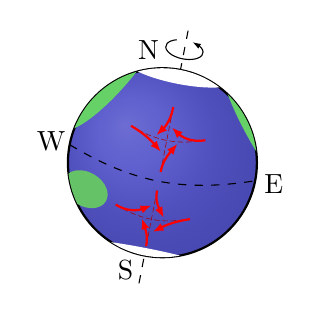
\begin{tikzpicture}
  \def\E{1.2}
  \coordinate (O) at (0,0);
  
  % EARTH
  \draw[dashed,rotate=-11] (0,-1.3*\E) -- (0,1.45*\E);
  \fill[blue!70!black!70] (0,0) circle (1.2);
  \draw[thick,ball color=blue!70!black!40,fill opacity=0.2] (0,0) circle (\E);
  \begin{scope}[rotate=-11]
    \draw[-{Latex[length=3,width=2,flex'=1]}] (0,1.22*\E)++(120:{0.2*\E} and 0.1*\E) arc(120:430:{0.2*\E} and 0.1*\E);
    \clip (0,0) circle (\E);
    \fill[white] (0,\E) ellipse ({0.6*\E} and {0.15*\E});
    \fill[white] (0,-\E) ellipse ({0.8*\E} and {0.08*\E});
    \fill[green!70!black!60,rotate=-30] (160:1.1*\E) ellipse ({0.2*\E} and {0.8*\E});
    \fill[green!70!black!60,rotate=40] (-10:1.14*\E) ellipse ({0.2*\E} and {0.9*\E});
    \fill[green!60!black!60,very thick,rotate=-20] % Australia
      (230:0.86*\E) ellipse ({0.25*\E} and {0.18*\E});
    \draw[dashed] (-\E,0) to[out=-20,in=-160] (\E,0);
    
    % CORIOLIS
    \draw[myred,mydashed,very thin] (0,-0.1*\E) coordinate (NS) --++ (0, 0.70*\E) coordinate (NN);
    \draw[myred,mydashed,very thin] (0,-0.3*\E) coordinate (SN) --++ (0,-0.60*\E) coordinate (SS);
    \draw[myred,mydashed,very thin] (-0.4*\E,0.32*\E) coordinate (NW) to[out=-20,in=-160]++ (0.8*\E,0) coordinate (NE);
    \draw[myred,mydashed,very thin] (-0.4*\E,-0.53*\E) coordinate (SW) to[out=-20,in=-160]++ (0.8*\E,0) coordinate (SE);
    \draw[myarr,red] (NN) to[out=-90,in=  50]++ (-110:0.35*\E); % northern hemisphere
    \draw[myarr,red] (NS) to[out= 90,in=-120]++ (  70:0.35*\E);
    \draw[myarr,red] (SN) to[out=-90,in= 130]++ ( -65:0.30*\E); % southern hemisphere
    \draw[myarr,red] (SS) to[out= 90,in= -60]++ ( 110:0.30*\E);
    \draw[myarr,red] (NE) to[out=200,in= -40]++ (170:0.38*\E); % northern hemisphere
    \draw[myarr,red] (NW) to[out=-20,in= 140]++ (-30:0.42*\E);
    \draw[myarr,red] (SE) to[out=200,in=  40]++ (210:0.42*\E); % southern hemisphere
    \draw[myarr,red] (SW) to[out=-20,in=-140]++ ( 10:0.38*\E);
  \end{scope}
  
  \node at (108-11:1.2*\E) {N};
  \node at (180-11:1.2*\E) {W};
  \node at (   -11:1.2*\E) {E};
  \node at (-98-11:1.2*\E) {S};
  
\end{tikzpicture}


\end{document}